\chapter{Технологическая часть}

В данной части приводится обоснование выбора СУБД и средств реализации приложения для взаимодействия с базой данных. Также приводится реализация создания таблиц базы данных, реализация ролевой модели на уровне базы данных и реализация триггера. Кроме того описаны методы тестирования разработанного функционала и приведена реализация интерфейса доступа к базе данных.

\section{Выбор системы управления базами данных}

Чтобы выбрать СУБД необходимо рассмотреть следующие критерии:
\begin{itemize}
    \item бесплатное и открытое программное обеспечение;
    \item поддержка процедурных расширений языка SQL;
    \item наличие личного опыта работы.
\end{itemize}

\begin{table}[H]
    \caption{\label{tbl:dbms}}
	\resizebox{\textwidth}{!}{
	\def\arraystretch{1}
    \begin{tabular}{|l|c|c|c|}
    \hline
    \begin{tabular}[c]{@{}l@{}}Система управления \\ базами данных\end{tabular} &
      \multicolumn{1}{l|}{\begin{tabular}[c]{@{}l@{}}Бесплатное и открытое \\ программное обеспечение\end{tabular}} &
      \multicolumn{1}{l|}{\begin{tabular}[c]{@{}l@{}}Поддержка процедурных \\ расширений языка SQL\end{tabular}} &
      \multicolumn{1}{l|}{\begin{tabular}[c]{@{}l@{}}Наличие личного \\ опыта работы\end{tabular}} \\ \hline
    PostgreSQL~\cite{postgres} & + & + & + \\ \hline
    Oracle~\cite{oracle}     & - & + & - \\ \hline
    SQLite~\cite{sqlite}     & + & + & - \\ \hline
    \end{tabular}
    }
\end{table}

По таблице \ref{tbl:dbms} можно сделать вывод, что наиболее подходящей СУБД для данной работы является PostgreSQL.

\section{Выбор объектного хранилища}

Объектное хранилище --- это тип системы хранения данных, предназначенный для управления большими объемами неструктурированной информации, такой как мультимедийные файлы, бэкапы, лог-файлы, документы и другие типы данных. Вместо традиционной файловой системы или реляционной базы данных, объектное хранилище организует данные в виде <<объектов>>.

Для хранения файлов с материалами создаваемых преподавателями курсов необходимо использовать объектное хранилище. При этом в базе данных должны храниться ссылки на получение данных файлов пользователем курса. 

Amazon S3~\cite{s3} --- одно из самых популярных облачных хранилищ с поддержкой API, множеством классов хранения и глобальной инфраструктурой для высокой доступности. Данное хранилище не доступно на территории РФ, поэтому использование его в данной работе невозможно. 

Google Cloud Storage~\cite{google-cloud} --- это облачная служба хранения данных от Google, предназначенная для хранения и управления большими объёмами неструктурированных данных. Это объектное хранилище, которое позволяет загружать, сохранять и извлекать данные любого типа, например, мультимедийные файлы, резервные копии, журналы, архивы, документы и многое другое. Данное хранилище доступно в РФ, однако услуги, предоставляемые компанией платные.

MinIO~\cite{minio} --- это программное обеспечение с открытым исходным кодом, которое позволяет создавать объектные хранилища, совместимые с API Amazon S3. MinIO часто используется для развертывания облачных хранилищ на локальных серверах, в частных или гибридных облаках. 

Учитывая доступность объектных хранилищ на территории РФ, их стоимость и наличие личного опыта работы, было выбрано хранилище MinIO для взаимодействия с файлами материалов курсов преподавателей. 

\section{Средства реализации}

В данной работе использованы следующие средства реализации:
\begin{itemize}
    \item язык программирования Golang~\cite{go};
    \item СУБД PostgreSQL~\cite{postgres};
    \item расширение языка SQL PL/pgSQL~\cite{pgsql};
    \item автоматизация развертывания реализована с помощью Docker~\cite{docker}.
\end{itemize}

Доступ к базе данных реализован в виде консольного интерфейса. Тестирование функционала проводилось с помощью встроенной программы go test~\cite{go-test}.

\section{Создание таблиц базы данных}

В листинге \ref{lst:scheme.sql} приведена реализация создания таблиц для сущностей предметной области.

\section{Создание ролей базы данных}

В листинге \ref{lst:roles.sql} приведена реализация создания ролей базы данных.

\pagebreak
\section{Реализация триггера}

В листинге \ref{lst:trigger.sql} приведена реализация триггера для пересчета средней оценки курса.

\includelisting
    {trigger.sql}
    {Реализация триггера}

\pagebreak
\section{Интерфейс доступа к базе данных}

В листинге \ref{lst:interface.txt} приведен пример пользовательского интерфейса.

\includelisting
    {interface.txt}
    {Консольный интерфейс приложения}

\section{Тестирование разработанного функционала}

В процессе тестирования были использованы два подхода: модульное тестирование и интеграционное. Модульное тестирование проводилось с помощью стандартного пакета testing~\cite{go-test} языка golang. Для изоляции сервисного слоя приложения использовался подход mock тестирования~\cite{mock-testing} и библиотека Mockery~\cite{mockery}.

Интеграционное тестирование уровня доступа к базе данных проводилось с использованием библиотеки Testcontainers~\cite{testcontainers}. 

На рисунке \ref{img:tests} изображены результаты пройденных тестов и их количество.

\begin{figure}[H]
	\centering
	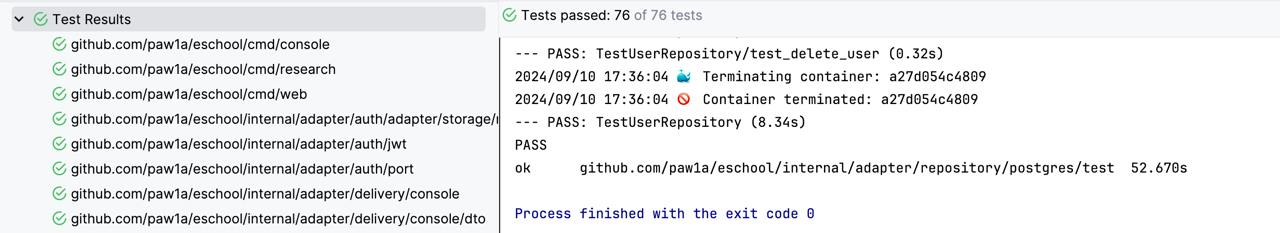
\includegraphics[height=0.12\textheight]{inc/img/tests.jpeg}
	\caption{Результаты пройденных тестов разработанного функционала}
	\label{img:tests}
\end{figure}

\section{Вывод из технолгической части}

В данной части была выбрана используемая СУБД и средства реализации приложения для взаимодействия с базой данных, приведена реализация создания таблиц базы данных, реализация ролевой модели на уровне базы данных и триггера. Были представлены методы тестирования разработанного функционала и пример реализации интерфейса доступа к базе данных.
